%This is a LaTeX template for homework assignments
\documentclass[8pt]{article}
\usepackage[top=1in, bottom=1in, left=1.1in, right=1.1in]{geometry}
\usepackage[utf8]{inputenc}
\usepackage{amsmath}
\usepackage{CJK}
\usepackage{enumerate}
\usepackage{ifthen}
\usepackage{listings}
\lstset{
  language=python,
  keywordstyle=\color{blue!70},
  frame=single,
  basicstyle=\ttfamily,
  commentstyle=\color{red},
  breakindent=0pt,
  rulesepcolor=\color{red!20!green!20!blue!20},
  rulecolor=\color{black},
  tabsize=4,
  numbersep=5pt,
  showstringspaces=false,
  breaklines=true,
  backgroundcolor=\color{red!10},
  showspaces=false,
  showtabs=false,
  extendedchars=false,
  escapeinside=``,
  frame=no,
}

\usepackage{fourier}
\usepackage{pgf}
\usepackage{tikz}
\usetikzlibrary{calc}
\usetikzlibrary{arrows,snakes,backgrounds,shapes,shadows}
\usetikzlibrary{matrix,fit,positioning,decorations.pathmorphing}



\newcommand{\tf}{\ttfamily}


\newlength{\la}
\newlength{\lb}
\newlength{\lc}
\newlength{\ld}
\newlength{\lhalf}
\newlength{\lquarter}
\newlength{\lmax}
\newcommand{\xx}[4]{\\[.5pt]%
\settowidth{\la}{A.~#1~~}
\settowidth{\lb}{B.~#2~~}
\settowidth{\lc}{C.~#3~~}
\settowidth{\ld}{D.~#4~~}
%%
\ifthenelse{\lengthtest{\la>\lb}}
{\setlength{\lmax}{\la}}
{\setlength{\lmax}{\lb}}
\ifthenelse{\lengthtest{\lmax<\lc}}
{\setlength{\lmax}{\lc}}
{}
\ifthenelse{\lengthtest{\lmax<\ld}}
{\setlength{\lmax}{\ld}}
{}
%%
\setlength{\lhalf}{0.5\linewidth}
\setlength{\lquarter}{0.25\linewidth}
%%
\ifthenelse{\lengthtest{\lmax>\lhalf}}
{\noindent{}A.~#1 \\ B.~#2 \\ C.~#3 \\ D.~#4 }
{
\ifthenelse{\lengthtest{\lmax>\lquarter}}
{\noindent
\makebox[\lhalf][l]{A.~#1~~}%
\makebox[\lhalf][l]{B.~#2~~}\\
\makebox[\lhalf][l]{C.~#3~~}%
\makebox[\lhalf][l]{D.~#4~~}
}%
{\noindent
\makebox[\lquarter][l]{A.~#1~~}%
\makebox[\lquarter][l]{B.~#2~~}%
\makebox[\lquarter][l]{C.~#3~~}%
\makebox[\lquarter][l]{D.~#4~~}
}
}
}



\begin{document}
\begin{CJK}{UTF8}{gkai}
\begin{center}
{\Large \bf  武汉大学数学与统计学院2017-2018学年第一学期期末考试\\[0.1in]
  数据结构与算法(B卷答案)} \vspace{0.1in}

\end{center}


\begin{enumerate} %\line(1,0){20}
\item (20分)~Python相关
  \begin{enumerate}
  \item (5分)
    \begin{lstlisting}
sum = 0
n = 99
while n > 0:
    sum = sum + n
    n = n - 2
print sum      
    \end{lstlisting}
  \item (5分)
    \begin{lstlisting}
[7, 9]
[1, 5]
[5, 7, 9]
ABC
ACEG
    \end{lstlisting}
  \item (5分)
\begin{lstlisting}
[s.lower() for s in alist]
  \end{lstlisting}
\item (5分)
  \begin{lstlisting}
PI = 3.1415926    
class Circle(object):
    def __init__(self, ratio):
        self.ratio = ratio
    def area(self):
        return PI * self.ratio**2
    def circum(self):
        return 2 * PI * self.ratio
  \end{lstlisting}    
  \end{enumerate}
\item (15分)~
  \begin{lstlisting}
    current !=None and not found and not stop
    current = current.next
    current =self.head
    temp.next = self.head
    self.head = temp
  \end{lstlisting}
\item (15分)~
  \begin{lstlisting}
    stack.push(int(token))
    operand2 = stack.pop()
    operand1 = stack.pop()
    result = doMath(token,operand1,operand2)
    stack.push(result)
  \end{lstlisting}
\item (15分)~
  \begin{enumerate}
  \item (5分)~
    \begin{lstlisting}
      def postorder(self):
          if tree:
              postorder(self.lchild)
              postorder(self.rchild)
              print(self.data)
    \end{lstlisting}
  \item (10分)~
    \begin{lstlisting}
      def insert(self, data):
        if data < self.data:
            if self.lchild:
                self.lchild.insert(data)
            else:
                tree = BinarySearchTree(data)
                self.lchild = tree
        elif data > self.data:
            if self.rchild:
                self.rchild.insert(data)
            else:
                tree = BinarySearchTree(data)
                self.rchild = tree
      \end{lstlisting}
  \end{enumerate}
\item (20分)~
  \begin{enumerate}
  \item (10分)~
    \begin{lstlisting}
def binarySearch(alist, item):
    first = 0
    last = len(alist)-1
    found = False
    
    while first <= last and not found:
        mid = (first + last)//2
        if alist[mid] == item:
            found = True
        else:
            if item < alist[mid]:
                last = mid-1
            else:
                first = mid+1
    return found
  \end{lstlisting}
  \item (10分)
    \begin{lstlisting}
def selectionSort(alist):
   for fillslot in range(len(alist)-1, 0, -1):
       positionOfMax = 0
       for location in range(1, fillslot+1):
           if alist[location] > alist[positionOfMax]:
               positionOfMax = location

       temp = alist[fillslot]
       alist[fillslot] = alist[positionOfMax]
       alist[positionOfMax] = temp
    \end{lstlisting}
  \end{enumerate}
\item (15分)~给定无向图
  \begin{figure}[htbp]
    \centering
  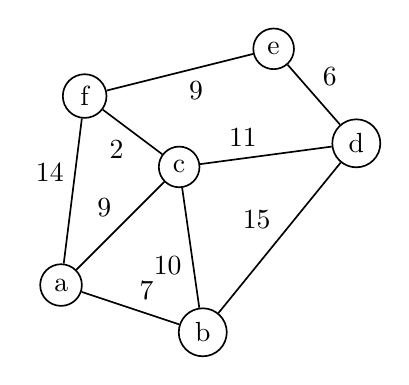
\begin{tikzpicture}[scale=1.5,node distance=3cm,semithick,inner sep=3pt,bend angle=45,auto]
    % \draw[help lines] (0,-1) grid (7,3);
    \node[circle,draw]   (a) at (0,0)  {a};
    \node[circle,draw]   (b) at (1.2,-.4)   {b};
    \node[circle,draw]   (c) at (1.0,1.0) {c};
    \node[circle,draw]   (d) at (2.5,1.2){d};
    \node[circle,draw]   (e) at (1.8,2.0){e};
    \node[circle,draw]   (f) at (0.2,1.6){f};
    \path
    (a) edge node{ 7}      (b)
        edge node{ 9}      (c)
        edge node{14}      (f)
    (b) edge node{10}      (c)
        edge node{15}      (d)
    (c) edge node{ 2}      (f)
        edge node{11}      (d)
    (e) edge node{ 9}      (f)
        edge node{ 6}      (d);
  \end{tikzpicture}
\end{figure}
\begin{enumerate}
  \item (5分)
    
    \begin{figure}[htbp]
      \centering
      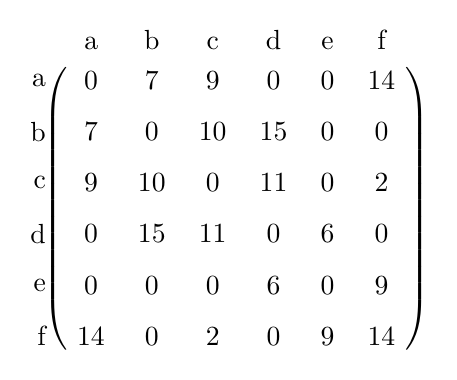
\begin{tikzpicture}[scale=1.5,node distance=3cm,semithick,inner sep=1pt,bend angle=45,auto]
        \matrix (am)  [matrix of math nodes,left delimiter=(,right delimiter=),row sep=10pt,column sep=10pt,right] 
        {
          0 & 7 & 9 & 0 & 0 &14\\
          7 & 0 &10 &15 & 0 & 0\\
          9 & 10& 0 &11 & 0 & 2\\
          0 & 15&11 & 0 & 6 & 0\\
          0 & 0 & 0 & 6 & 0 & 9\\
          14& 0 & 2 & 0 & 9 &14\\
        };
        \node at (am-1-1) [above=10pt] {a}; 
        \node at (am-1-2) [above=10pt] {b};       
        \node at (am-1-3) [above=10pt] {c};       
        \node at (am-1-4) [above=10pt] {d};
        \node at (am-1-5) [above=10pt] {e};
        \node at (am-1-6) [above=10pt] {f};
        \node at (am-1-1) [left=15pt] {a}; 
        \node at (am-2-1) [left=15pt] {b};       
        \node at (am-3-1) [left=15pt] {c};       
        \node at (am-4-1) [left=15pt] {d};             
        \node at (am-5-1) [left=15pt] {e};             
        \node at (am-6-1) [left=15pt] {f};             
      \end{tikzpicture}
    \end{figure}
  \item (5分)
    \begin{lstlisting}
{'a': 3, 'b': 3, 'c': 4, 'd': 3, 'e': 2, 'f': 3}     
    \end{lstlisting}
  \item (5分)~
    \begin{lstlisting}[title=深度优先]
a, b, c, d, e, f          
    \end{lstlisting}
    \begin{lstlisting}[title=广度优先]
a, b, c, f, d, e
    \end{lstlisting}

\end{enumerate}
\end{enumerate}



\end{CJK}
\end{document}
